\section{Propriétés réfléctives des élements à capturer}
Durant ses activités, le système observera principalement les élements suivants:
\begin{listage}
    1. Les hydrocarbures\\
    2. Le béton\\
    3. Le goudron
\end{listage}
On m'informant sur les méthodes de détection déjà existante des hydrocarbures, j'ai constaté que l'intégralité d'entre eux fonctionnent
par ultraviolet (mesure de fluoresence) et par infrarouge. Je vais donc m'informer sur la réaction des éléments susmentionné suivant l'exposition à différentes longueurs d'ondes.
\subsection{Hydrocarbures}
Les principaux hydrocarbures traités par les pompiers durant leurs interventions sont les suivants:
\begin{listage}
    1. L'huile de moteur\\
    2. L'huile hydraulique (tracteur)\\
    3. L'essence \cite{TotalEnergies}\\
    4. Le diesel \cite{TotalEnergies}
\end{listage}
Les éléments principaux qui les composent sont les suivants:
\begin{listage}
    - Les alcènes\\
    - Les alcanes\\
    - Les hydrocarbures aromatiques
\end{listage}
Divers travaux \cite{Hydrocarbures} traitent des spectres IR des hydrocarbures, mettant en relation la transmittance des éléments en fonction de la longueur d'onde.
Tirés desdits travaux, les graphiques suivants délivres des informations utiles sur la problèmatique du projet.

\begin{figure}[H]
    \centering
    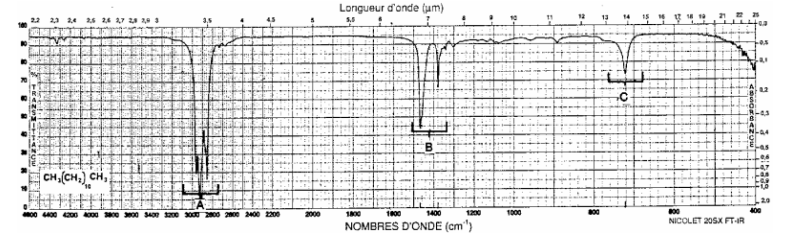
\includegraphics[height=7cm,angle=90]{assets/figures/alcanes1.png}
    \caption{Alcanes - spectre IR du dodécane \cite{Hydrocarbures}}
\end{figure}

\begin{figure}[H]
    \centering
    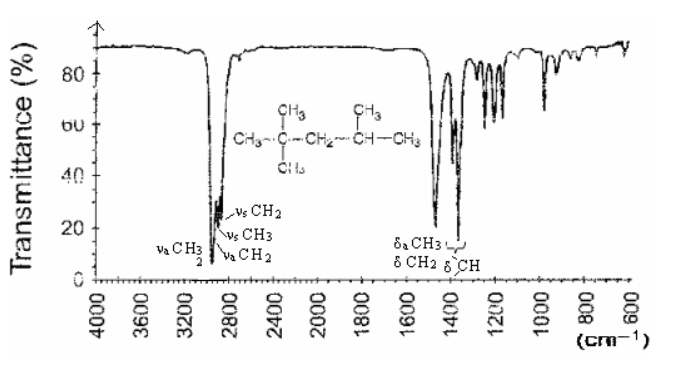
\includegraphics[height=6cm,angle=90]{assets/figures/alcanes2.png}
    \caption{Alcanes - spectre IR du triméthyl-pentane \cite{Hydrocarbures}}
\end{figure}

\begin{figure}[H]
    \centering
    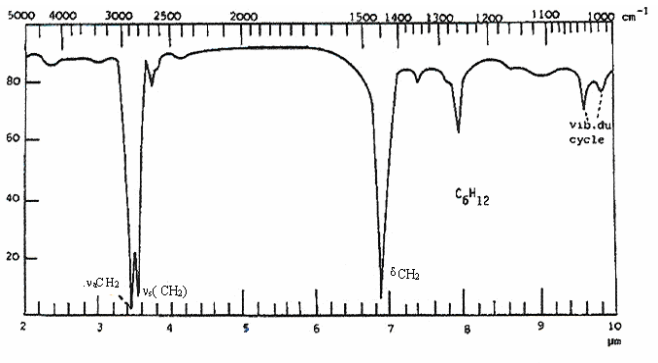
\includegraphics[height=5cm,angle=90]{assets/figures/alcanes3.png}
    \caption{Alcanes - spectre IR du cycloalcanes \cite{Hydrocarbures}}
\end{figure}

\begin{figure}[H]
    \centering
    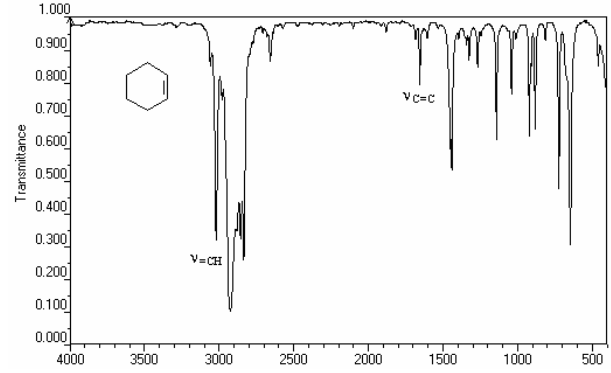
\includegraphics[height=5cm,angle=90]{assets/figures/alcenes1.png}
    \caption{Alcènes - spectre IR du cyclohexène \cite{Hydrocarbures}}
\end{figure}

\begin{figure}[H]
    \centering
    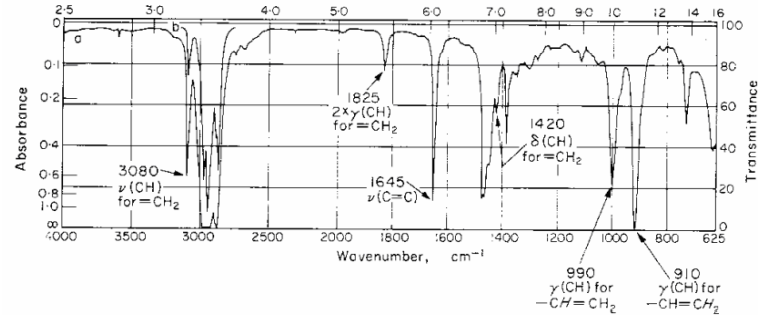
\includegraphics[height=5cm,angle=90]{assets/figures/alcenes2.png}
    \caption{Alcanes - spectre IR du  1-octène à l’état liquide\cite{Hydrocarbures}}
\end{figure}

\begin{figure}[H]
    \centering
    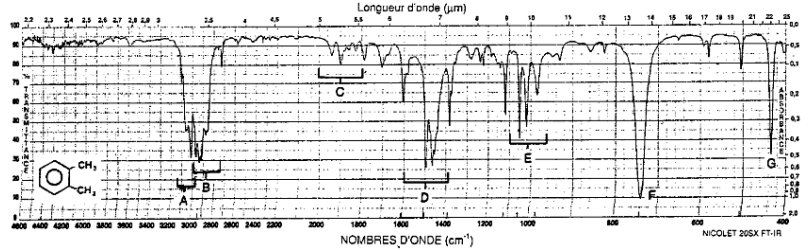
\includegraphics[height=5cm,angle=90]{assets/figures/aromatique.png}
    \caption{Aromatique - spectre IR du o-xylène \cite{Hydrocarbures}}
\end{figure}

\newpage
La transmittance indiquée sur l'axe de l'ordonnée représente l'inverse de l'absorbption, c'est à dire que si la transmittance est faible, la lumière
est "très" absorbée par l'hydrocarbure et inversement, si la transmittance est élevée, la lumière est "peu" absorbée par l'hydrocarbure, la laissant ainsi traverser.
Nous observons un point commun pour les trois types d'hydrocarbures, il s'agit des pics d'absorbptions aux alentours de \underline{3000 \si{\per\centi\metre}}, ce qui correspond à \underline{3300 \si{\nano\metre}}.\\
Pour cette longueur d'onde spécifique, la transmittance globale se trouve entre \underline{5 et 30\%}.

\subsection{Béton}

\subsection{Goudron}
On retrouve des hydrocarbures dans la composition du goudron, ceux-ci étant similaires aux hydrocarbures à détecter, le spectre IR pourrait nous indiquer des problèmes de détection pour la classification ...

\subsection{Bitume}
Une bonne source ici: \cite{Bitume}
\\

\subsection{Analyse}
On observe que les diverses élements qui seront vus par la caméra ont une variation du taux d'absorptions face aux longueurs d'onde avoisinant les
3300 \si{\nano\metre}, mais à différents ordres de grandeurs. Là ou les hydrocarbures absorbent jusqu'à 95\% des ondes, les routes en absorbent "seulement" jusqu'à 50\%.
En se basant sur ceci, il devrait être possible de faire une différenciation par l'intermédiaire d'un capteur adapté.\\
Selon les normes \Gls{iso} 20473:2007 \cite{ISO}, cette longueur d'onde se trouve parmi les \Gls{mir}.\\
\begin{figure}[H]
    \centering
    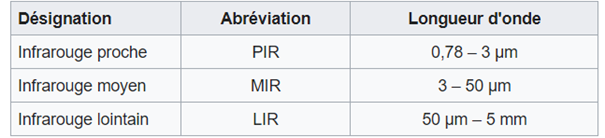
\includegraphics[width=13cm]{assets/figures/gamme_infra.png}
    \caption{Classification des \Gls{ir} selon les normes \Gls{iso} 20473:2007 \cite{ISO}}
\end{figure}
